\documentclass[10pt]{beamer}\usepackage[]{graphicx}\usepackage[]{color}
% maxwidth is the original width if it is less than linewidth
% otherwise use linewidth (to make sure the graphics do not exceed the margin)
\makeatletter
\def\maxwidth{ %
  \ifdim\Gin@nat@width>\linewidth
    \linewidth
  \else
    \Gin@nat@width
  \fi
}
\makeatother

\definecolor{fgcolor}{rgb}{0.345, 0.345, 0.345}
\newcommand{\hlnum}[1]{\textcolor[rgb]{0.686,0.059,0.569}{#1}}%
\newcommand{\hlstr}[1]{\textcolor[rgb]{0.192,0.494,0.8}{#1}}%
\newcommand{\hlcom}[1]{\textcolor[rgb]{0.678,0.584,0.686}{\textit{#1}}}%
\newcommand{\hlopt}[1]{\textcolor[rgb]{0,0,0}{#1}}%
\newcommand{\hlstd}[1]{\textcolor[rgb]{0.345,0.345,0.345}{#1}}%
\newcommand{\hlkwa}[1]{\textcolor[rgb]{0.161,0.373,0.58}{\textbf{#1}}}%
\newcommand{\hlkwb}[1]{\textcolor[rgb]{0.69,0.353,0.396}{#1}}%
\newcommand{\hlkwc}[1]{\textcolor[rgb]{0.333,0.667,0.333}{#1}}%
\newcommand{\hlkwd}[1]{\textcolor[rgb]{0.737,0.353,0.396}{\textbf{#1}}}%
\let\hlipl\hlkwb

\usepackage{framed}
\makeatletter
\newenvironment{kframe}{%
 \def\at@end@of@kframe{}%
 \ifinner\ifhmode%
  \def\at@end@of@kframe{\end{minipage}}%
  \begin{minipage}{\columnwidth}%
 \fi\fi%
 \def\FrameCommand##1{\hskip\@totalleftmargin \hskip-\fboxsep
 \colorbox{shadecolor}{##1}\hskip-\fboxsep
     % There is no \\@totalrightmargin, so:
     \hskip-\linewidth \hskip-\@totalleftmargin \hskip\columnwidth}%
 \MakeFramed {\advance\hsize-\width
   \@totalleftmargin\z@ \linewidth\hsize
   \@setminipage}}%
 {\par\unskip\endMakeFramed%
 \at@end@of@kframe}
\makeatother

\definecolor{shadecolor}{rgb}{.97, .97, .97}
\definecolor{messagecolor}{rgb}{0, 0, 0}
\definecolor{warningcolor}{rgb}{1, 0, 1}
\definecolor{errorcolor}{rgb}{1, 0, 0}
\newenvironment{knitrout}{}{} % an empty environment to be redefined in TeX

\usepackage{alltt}


%\input{slides_header.tex}
\usepackage{graphicx}
\usepackage{hyperref, url}
\hypersetup{colorlinks,citecolor=myorange,filecolor=red,linkcolor=brown,urlcolor=blue}

\usepackage{longtable,booktabs}
\usepackage{amssymb,amsmath}
\usepackage{animate}
\usepackage{subfig}
\usepackage{tikz}
\usetikzlibrary{shapes.geometric, arrows,shapes.symbols,decorations.pathreplacing}
\tikzstyle{startstop} = [rectangle, rounded corners, minimum width=3cm, minimum height=1cm, draw=black, fill=pinkish,text width=3.5cm]
\tikzstyle{startstop2} = [rectangle, rounded corners, minimum width=3cm, minimum height=1cm, draw=black, fill=background,text width=4.5cm]
\tikzstyle{startstop3} = [rectangle, rounded corners, minimum width=3cm, minimum height=1cm, draw=black, fill=beige,text width=3.0cm]
\tikzstyle{startstop4} = [rectangle, rounded corners, minimum width=3cm, minimum height=1cm, draw=black, fill=pinkish,text width=4.5cm]
\tikzstyle{io} = [trapezium, trapezium left angle=70, trapezium right angle=110, minimum width=2cm, minimum height=1cm, text centered, draw=black, fill=blue!30,text width=1.5cm]
\tikzstyle{process} = [rectangle, minimum width=1cm, minimum height=1cm, text centered, draw=black, fill=orange!30,text width=2cm]
\tikzstyle{decision} = [diamond, minimum width=2cm, minimum height=1cm, text centered, draw=black, fill=green!30]
\tikzstyle{arrow} = [thick,->,>=stealth]
\tikzstyle{both} = [thick,<->,>=stealth, red]


% used for tree of stats tests in 001-introduction
\tikzstyle{startstopstats} = [rectangle, rounded corners, minimum width=2cm, minimum height=.5cm,text centered, draw=black, fill=red!30]
\tikzstyle{iostats} = [trapezium, trapezium left angle=70, trapezium right angle=110, minimum width=2cm, minimum height=.5cm, text centered, draw=black, fill=blue!30]
\tikzstyle{processstats} = [rectangle, minimum width=1.5cm, minimum height=.5cm, text centered, draw=black, fill=orange!30]
\tikzstyle{processbigstats} = [rectangle, minimum width=1.5cm, minimum height=.5cm, text centered, draw=black, fill=orange!30,text width=1.6cm]
\tikzstyle{decisionstats} = [rectangle, minimum width=1cm, minimum height=1cm, text centered, draw=black, fill=green!30,text width=1.6cm]
\tikzstyle{decisionbigstats} = [rectangle, minimum width=1cm, minimum height=1cm, text centered, draw=black, fill=yellow!30,text width=2cm]

\usepackage{pifont}% http://ctan.org/pkg/pifont
\newcommand{\cmark}{\ding{51}}%
\newcommand{\xmark}{\ding{55}}%

\usepackage{ulem} % for strikeout

\usepackage{xcolor}
\usepackage{color, colortbl}
\definecolor{lightgray}{RGB}{200,200,200}
\definecolor{palegray}{RGB}{221,221,221}
\definecolor{myblue}{RGB}{0,89,179}
\definecolor{myorange}{rgb}{0.776,0.357,0.157}
\definecolor{gray}{RGB}{110,110,110}
\definecolor{darkgray}{RGB}{100,100,100}
\definecolor{lightgray}{RGB}{200,200,200}
\definecolor{palegray}{RGB}{221,221,221}
\definecolor{turquoise}{RGB}{81,193,188}
\definecolor{tomato}{RGB}{255,136,136}
\definecolor{mandarina}{RGB}{229,169,25}
\definecolor{foreground}{RGB}{81,141,193}
\definecolor{background}{RGB}{246,244,240}
\definecolor{highlight}{RGB}{229,169,25}
\definecolor{lowlight}{RGB}{200,200,200}
\definecolor{beige}{RGB}{255,255,240}
\definecolor{pinkish}{RGB}{255,223,247}
\definecolor{darktangerine}{rgb}{1.0, 0.66, 0.07}
\definecolor{deepink}{RGB}{255,20,147}
%\usepackage{shadethm}
%\colorlet{shadecolor}{blue!15}
%\colorlet{shadecolor}{palegray}
%\setlength{\shadeboxrule}{.4pt}

%\newshadetheorem{thm}{Theorem}
%\newshadetheorem{defm}{Definition}
%\newshadetheorem{exm}{Exercise}
%\newshadetheorem{remarkm}{Remark}
%\definecolor{shadethmcolor}{HTML}{EDF8FF}
%\definecolor{shadethmcolor}{RGB}{221,221,221}
%\definecolor{shaderulecolor}{HTML}{45CFFF}
%\definecolor{shaderulecolor}{RGB}{0,89,179}
%\setlength{\shadeboxrule}{.4pt}



\usepackage{epsfig}

\newcommand{\code}[1]{\texttt{#1}}
\newcommand{\blue}[1]{\textcolor{blue}{#1}}
\newcommand{\red}[1]{\textcolor{red}{#1}}

\usepackage{comment}

\makeatletter

\def \iqsssectiontitleheader {}

\newcommand{\iqsssectiontitle}[1]{
	\def \iqsssectiontitleheader{#1}
}

\@ifundefined{insertmainframenumber}
{%
	% \insertmainframenumber not defined
	\newcommand{\insertmainframenumber}{\inserttotalframenumber}
}
{%
	% \insertmainframenumber already defined
}%


\AtBeginSection[]{
	\title{\insertsectionhead}
	{
		%\definecolor{white}{RGB}{140,193,250}
		%\definecolor{white}{RGB}{200,200,200}
		%\definecolor{white}{RGB}{242,244,247}
		\definecolor{white}{RGB}{0,89,179}
		%\definecolor{iqss@orange}{rgb}{1,1,1}
		\ifnum \insertmainframenumber > \insertframenumber
		%\setbeamercolor{background canvas}{bg=myblue}
		%\setbeamercolor{normal text}{fg=black,bg=white}
		%\setbeamercolor{frametitle}{fg=red}
		%\setbeamercolor{section in toc}{fg=myblue, bg=white}
		%\setbeamercolor{subsection in toc}{fg=myblue, bg=white}
		\frame{
			\frametitle{\iqsssectiontitleheader}
			\tableofcontents[currentsection]
		}
		\else
		\frame{
			\frametitle{Backup Slides}
			\tableofcontents[sectionstyle=shaded/shaded,subsectionstyle=shaded/shaded/shaded]
		}
		\fi
	}
}
\makeatother
%\graphicspath{{/home/sahir/git_repositories/EPIB607/resources/assets/slides/figure/}}


\usepackage{fontspec}
%\setsansfont{Fira Sans}
%\setmonofont{Fira Mono}
%\setsansfont[ItalicFont={Fira Sans Light Italic},BoldFont={Fira Sans},BoldItalicFont={Fira Sans Italic}]{Fira Sans Light}
%\setmonofont[BoldFont={Fira Mono Medium}]{Fira Mono}

\def\installpath{/usr/local/share/texmf/fonts/opentype/libertinus/}
\setmainfont{LibertinusSerif}[
UprightFont    = *-Regular,
BoldFont       = *-Bold,
ItalicFont     = *-Italic,
BoldItalicFont = *-BoldItalic,
Ligatures      = TeX,
Extension      = .otf,
Path           = \installpath/
]

\setsansfont{LibertinusSerif}[
UprightFont    = *-Regular,
BoldFont       = *-Bold,
ItalicFont     = *-Italic,
BoldItalicFont = *-BoldItalic,
Ligatures      = TeX,
Extension      = .otf,
Path           = \installpath/
]


%\setmonofont{LibertinusSerif}[
%UprightFont    = *-Regular,
%BoldFont       = *-Bold,
%ItalicFont     = *-Italic,
%BoldItalicFont = *-BoldItalic,
%Ligatures      = TeX,
%Extension      = .otf,
%Path           = \installpath/
%]






\newcommand\Wider[2][3em]{%
	\makebox[\linewidth][c]{%
		\begin{minipage}{\dimexpr\textwidth+#1\relax}
			\raggedright#2
		\end{minipage}%
	}%
}


\newcommand {\framedgraphic}[1] {
	\begin{figure}
		\centering
		\includegraphics[width=\textwidth,height=0.9\textheight,keepaspectratio]{#1}
	\end{figure}
}


\newcommand {\framedgraphiccaption}[2] {
	\begin{figure}
		\centering
		\includegraphics[width=\textwidth,height=0.8\textheight,keepaspectratio]{#1}
		\caption{#2}
	\end{figure}
}




\setbeamercolor{itemize item}{fg=myblue}
\setbeamercolor{itemize subitem}{fg=myorange}
%\setbeamertemplate{itemize item}[square]
\setbeamertemplate{itemize item}[circle]
\setbeamertemplate{itemize subitem}[triangle]
\setbeamertemplate{blocks}[rounded][shadow=true]
\setbeamercolor{block body alerted}{bg=alerted text.fg!10}
\setbeamercolor{block title alerted}{bg=alerted text.fg!20}
\setbeamercolor{block body}{bg=structure!10}
\setbeamercolor{block title}{bg=structure!20}
\setbeamercolor{block body example}{bg=green!10}
\setbeamercolor{block title example}{bg=green!20}


\makeatletter
\newenvironment<>{proofs}[1][\proofname]{%
	\par
	\def\insertproofname{#1\@addpunct{.}}%
	\usebeamertemplate{proof begin}#2}
{\usebeamertemplate{proof end}}
\newenvironment<>{proofc}{%
	\setbeamertemplate{proof begin}{\begin{block}{}}
		\par
		\usebeamertemplate{proof begin}}
	{\usebeamertemplate{proof end}}
	\newenvironment<>{proofe}{%
		\par
		\pushQED{\qed}
		\setbeamertemplate{proof begin}{\begin{block}{}}
			\usebeamertemplate{proof begin}}
		{\popQED\usebeamertemplate{proof end}}
\makeatother


\makeatletter
\newenvironment<>{exams}[1][\proofname]{%
	\par
	\def\insertproofname{#1\@addpunct{.}}%
	\usebeamertemplate{example begin}#2}
{\usebeamertemplate{example end}}
\newenvironment<>{examc}{%
	\setbeamertemplate{exam begin}{\begin{block}{}}
		\par
		\usebeamertemplate{exam begin}}
	{\usebeamertemplate{exam end}}
	\newenvironment<>{exame}{%
		\par
		\pushQED{\qed}
		\setbeamertemplate{exam begin}{\begin{block}{}}
			\usebeamertemplate{exam begin}}
		{\popQED\usebeamertemplate{exam end}}
		\makeatother

%\definecolor{mycolor}{HTML}{F7F8E0}
%\declaretheorem[shaded={bgcolor=mandarina}]{theo}
%\declaretheorem[shaded={bgcolor=mycolor}]{propo}
%\declaretheorem[shaded={bgcolor=green!80!black!30}]{remark}

%\setbeamertemplate{navigation symbols}{\usebeamercolor[fg]{title in head/foot}\usebeamerfont{title in head/foot}\insertframenumber}


%\setbeamertemplate{footline}{}

\beamertemplatenavigationsymbolsempty % toggle off if you want navigation symbols at the bottom

\setbeamertemplate{footline}
{ \usebeamercolor[fg]{page number in head/foot}%
	\usebeamerfont{page number in head/foot}%
	\hspace{1em}\insertsectionhead%
	\hfill%
	\insertframenumber\,/\,\hyperlinkappendixstart{\insertmainframenumber}
	\ifnum \thepage = \insertframeendpage{\small .}\else{\phantom{\small .}}\fi
	\hspace{1em}
	\vskip2pt%
}

%\newtheorem{proposition}[theorem]{Proposition}
%\newtheorem{exercise}[theorem]{Exercise}
%\newtheorem{remark}[theorem]{Remark}


\usepackage{amsthm}
\usepackage{thmtools}

\setbeamertemplate{theorems}[ams style] 
%\setbeamertemplate{theorems}[numbered] 
%\setbeamertemplate{corollary}[numbered] 
\newtheorem{proposition}{Proposition}
\newtheorem{exercise}{Exercise}
\newtheorem{remark}{Remark}
\newtheorem{exam}{Example}
%\newtheorem{proof}{Proof}
%\newtheorem{corollaries}[theorem]{Corollary}
\newcommand*{\theorembreak}{\usebeamertemplate{theorem end}\framebreak\usebeamertemplate{theorem begin}}



\setlength{\emergencystretch}{3em} % prevent overfull lines
\providecommand{\tightlist}{%
	\setlength{\itemsep}{0pt}\setlength{\parskip}{0pt}}

\newcommand\AddButton{%
	\setbeamertemplate{background canvas}{%
		\begin{tikzpicture}[remember picture,overlay]
		\node[anchor=west] at ([yshift=5pt,xshift=0.1em]current page.south west)
		{\hyperlink{toc}{\beamergotobutton{back to TOC}}};
		\end{tikzpicture}%
	}%
}


\titlegraphic{\hfill
\includegraphics[height=1cm]{/home/sahir/git_repositories/EPIB607/slides/mcgill_logo.png}}




\graphicspath{{/home/sahir/git_repositories/EPIB607/slides/figure/}}

%\let\oldShaded\Shaded
%\let\endoldShaded\endShaded
%\renewenvironment{Shaded}{\footnotesize\oldShaded}{\endoldShaded}

%\newcommand{\blue}[1]{\textcolor{blue}{#1}}
%\newcommand{\red}[1]{\textcolor{red}{#1}}


\usepackage{xparse}
\NewDocumentCommand\mylist{>{\SplitList{;}}m}
{
	\begin{itemize}
		\ProcessList{#1}{ \insertitem }
	\end{itemize}
}
\NewDocumentCommand\mynum{>{\SplitList{;}}m}
{
	\begin{enumerate}
		\ProcessList{#1}{ \insertitem }
	\end{enumerate}
}
\newcommand\insertitem[1]{\item #1}

\newcommand\FrameText[1]{%
	\begin{textblock*}{\paperwidth}(0pt,\textheight)
		\raggedright #1\hspace{.5em}
\end{textblock*}}
\IfFileExists{upquote.sty}{\usepackage{upquote}}{}
\begin{document}
	
	
	
	%\title{Introduction to Regression Trees}
	%\author{Sahir Bhatnagar \inst{1}}
	%\author[shortname]{Sahir Rai Bhatnagar, PhD Candidate (Biostatistics) }
	%\institute[shortinst]{Department of Epidemiology, Biostatistics and Occupational Health}
	
	\title{018 - Linear Regression}
	\author{EPIB 607 - FALL 2020}
	\institute{
		Sahir Rai Bhatnagar\\
		Department of Epidemiology, Biostatistics, and Occupational Health\\
		McGill University\\
		
		\vspace{0.1 in}
		
		\texttt{sahir.bhatnagar@mcgill.ca}\\
		%\texttt{\url{https://sahirbhatnagar.com/EPIB607/}}
	}
	
	\date{slides compiled on \today}
	
	\maketitle
	
	%\section{Objectives}
	
	\section{Example: Depths of the ocean}




\begin{frame}[fragile,plain]
\vspace*{-1.0in}
\textbf{1. Mean depth of the ocean}


\begin{knitrout}\tiny
\definecolor{shadecolor}{rgb}{0.969, 0.969, 0.969}\color{fgcolor}\begin{kframe}
\begin{alltt}
\hlkwd{head}\hlstd{(depths,} \hlkwc{n}\hlstd{=}\hlnum{3}\hlstd{)}
\end{alltt}
\begin{verbatim}
##           X      lon     lat  alt water South
## 26118 26118  157.559  8.8311 5044     1     0
## 29349 29349  -51.597 29.2888 5277     1     0
## 4391   4391 -133.031 13.6859 5032     1     0
\end{verbatim}
\begin{alltt}
\hlkwd{dim}\hlstd{(depths)}
\end{alltt}
\begin{verbatim}
## [1] 400   6
\end{verbatim}
\begin{alltt}
\hlstd{fit} \hlkwb{<-} \hlkwd{lm}\hlstd{(alt} \hlopt{~} \hlnum{1}\hlstd{,} \hlkwc{data} \hlstd{= depths)}
\hlkwd{print}\hlstd{(}\hlkwd{summary}\hlstd{(fit),} \hlkwc{signif.stars} \hlstd{= F)}
\end{alltt}
\begin{verbatim}
## Coefficients:
##             Estimate Std. Error t value Pr(>|t|)
## (Intercept)   3628.5       86.5      42   <2e-16
## 
## Residual standard error: 1730 on 399 degrees of freedom
\end{verbatim}
\end{kframe}
\end{knitrout}


\end{frame}


\begin{frame}[fragile,plain]
\vspace*{-.90551in}
%\scriptsize
\textbf{2. Difference of mean depth in north vs south hemisphere}

	
	
\begin{knitrout}\tiny
\definecolor{shadecolor}{rgb}{0.969, 0.969, 0.969}\color{fgcolor}\begin{kframe}
\begin{alltt}
\hlstd{fit} \hlkwb{<-} \hlkwd{lm}\hlstd{(alt} \hlopt{~} \hlstd{South,} \hlkwc{data} \hlstd{= depths)}
\hlkwd{print}\hlstd{(}\hlkwd{summary}\hlstd{(fit),} \hlkwc{signif.stars} \hlstd{= F)}
\end{alltt}
\begin{verbatim}
## Coefficients:
##             Estimate Std. Error t value Pr(>|t|)
## (Intercept)     3523        122   28.82   <2e-16
## South            211        173    1.22     0.22
## 
## Residual standard error: 1730 on 398 degrees of freedom
## Multiple R-squared: 0.00372,	Adjusted R-squared: 0.00122 
## F-statistic: 1.49 on 1 and 398 DF,  p-value: 0.223
\end{verbatim}
\begin{alltt}
\hlstd{stats}\hlopt{::}\hlkwd{t.test}\hlstd{(alt} \hlopt{~} \hlstd{South,} \hlkwc{data} \hlstd{= depths,} \hlkwc{var.equal} \hlstd{=} \hlnum{TRUE}\hlstd{)}
\end{alltt}
\begin{verbatim}
##  Two Sample t-test with alt by South 
## t = -1.2192, df = 398, p-value = 0.2235
## alternative hypothesis: true difference in means is not equal to 0 
## 95 percent confidence interval:
##  -550.58  129.08 
## sample estimates:
## mean in group 0 mean in group 1 
##          3523.1          3733.9
\end{verbatim}
\end{kframe}
\end{knitrout}
\end{frame}

\begin{frame}[fragile,plain]
	%\vspace*{-.0551in}
	%\scriptsize
%	\textbf{2. Difference of mean depth in north vs south hemisphere}

	
\begin{knitrout}\tiny
\definecolor{shadecolor}{rgb}{0.969, 0.969, 0.969}\color{fgcolor}\begin{kframe}
\begin{alltt}
\hlkwd{coef}\hlstd{(fit)}
\end{alltt}
\begin{verbatim}
## (Intercept)       South 
##     3523.11      210.75
\end{verbatim}
\begin{alltt}
\hlkwd{vcov}\hlstd{(fit)}
\end{alltt}
\begin{verbatim}
##             (Intercept)  South
## (Intercept)       14940 -14940
## South            -14940  29880
\end{verbatim}
\begin{alltt}
\hlkwd{confint}\hlstd{(fit)}
\end{alltt}
\begin{verbatim}
##               2.5 %  97.5 %
## (Intercept) 3282.82 3763.41
## South       -129.08  550.58
\end{verbatim}
\end{kframe}
\end{knitrout}
\end{frame}



\begin{frame}[fragile,plain]
	%	\vspace*{-0.2in}
	\small
	\textbf{2.2 Bootstrap CI for mean difference using canned function}
\begin{knitrout}\tiny
\definecolor{shadecolor}{rgb}{0.969, 0.969, 0.969}\color{fgcolor}\begin{kframe}
\begin{alltt}
\hlstd{pacman}\hlopt{::}\hlkwd{p_load}\hlstd{(car)}
\hlstd{betahat.boot} \hlkwb{<-} \hlstd{car}\hlopt{::}\hlkwd{Boot}\hlstd{(fit,} \hlkwc{R}\hlstd{=}\hlnum{999}\hlstd{)}
\hlkwd{head}\hlstd{(betahat.boot}\hlopt{$}\hlstd{t)}
\end{alltt}
\begin{verbatim}
##      (Intercept)   South
## [1,]      3577.0 115.734
## [2,]      3603.2 202.018
## [3,]      3521.5 250.253
## [4,]      3688.2  77.188
## [5,]      3574.3 203.502
## [6,]      3716.5 -88.660
\end{verbatim}
\begin{alltt}
\hlkwd{dim}\hlstd{(betahat.boot}\hlopt{$}\hlstd{t)}
\end{alltt}
\begin{verbatim}
## [1] 999   2
\end{verbatim}
\begin{alltt}
\hlstd{deltamuhat.boot} \hlkwb{<-} \hlstd{betahat.boot}\hlopt{$}\hlstd{t[,}\hlnum{2}\hlstd{]}
\hlkwd{median}\hlstd{(deltamuhat.boot)}
\end{alltt}
\begin{verbatim}
## [1] 204.45
\end{verbatim}
\begin{alltt}
\hlkwd{quantile}\hlstd{(deltamuhat.boot,} \hlkwc{probs} \hlstd{=} \hlkwd{c}\hlstd{(}\hlnum{0.025}\hlstd{,} \hlnum{0.975}\hlstd{))}
\end{alltt}
\begin{verbatim}
##    2.5%   97.5% 
## -141.92  553.28
\end{verbatim}
\end{kframe}

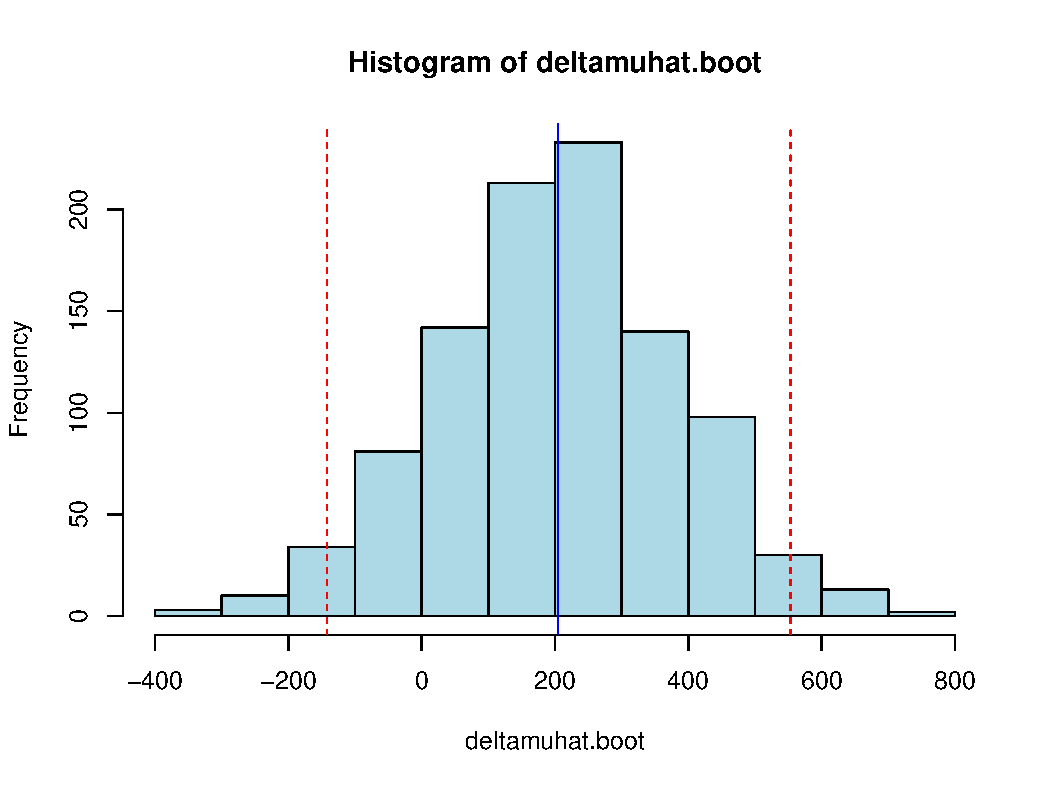
\includegraphics[width=0.35\textwidth]{figure/unnamed-chunk-6-1} \hfill{}



\end{knitrout}
	
\end{frame}


\begin{frame}[fragile,plain]
	%	\vspace*{-0.2in}
	\small
	\textbf{2.2 Bootstrap CI for mean difference using canned function (continued)}
\begin{knitrout}\tiny
\definecolor{shadecolor}{rgb}{0.969, 0.969, 0.969}\color{fgcolor}\begin{kframe}
\begin{alltt}
\hlkwd{summary}\hlstd{(betahat.boot)}
\end{alltt}
\begin{verbatim}
## 
## Number of bootstrap replications R = 999 
##             original bootBias bootSE bootMed
## (Intercept)     3523     3.65    140    3529
## South            211    -7.49    179     204
\end{verbatim}
\begin{alltt}
\hlkwd{confint}\hlstd{(betahat.boot)}
\end{alltt}
\begin{verbatim}
## Bootstrap bca confidence intervals
## 
##               2.5 %  97.5 %
## (Intercept) 3200.79 3782.23
## South       -127.46  569.08
\end{verbatim}
\begin{alltt}
\hlkwd{hist}\hlstd{(betahat.boot)}
\end{alltt}
\end{kframe}

{\centering 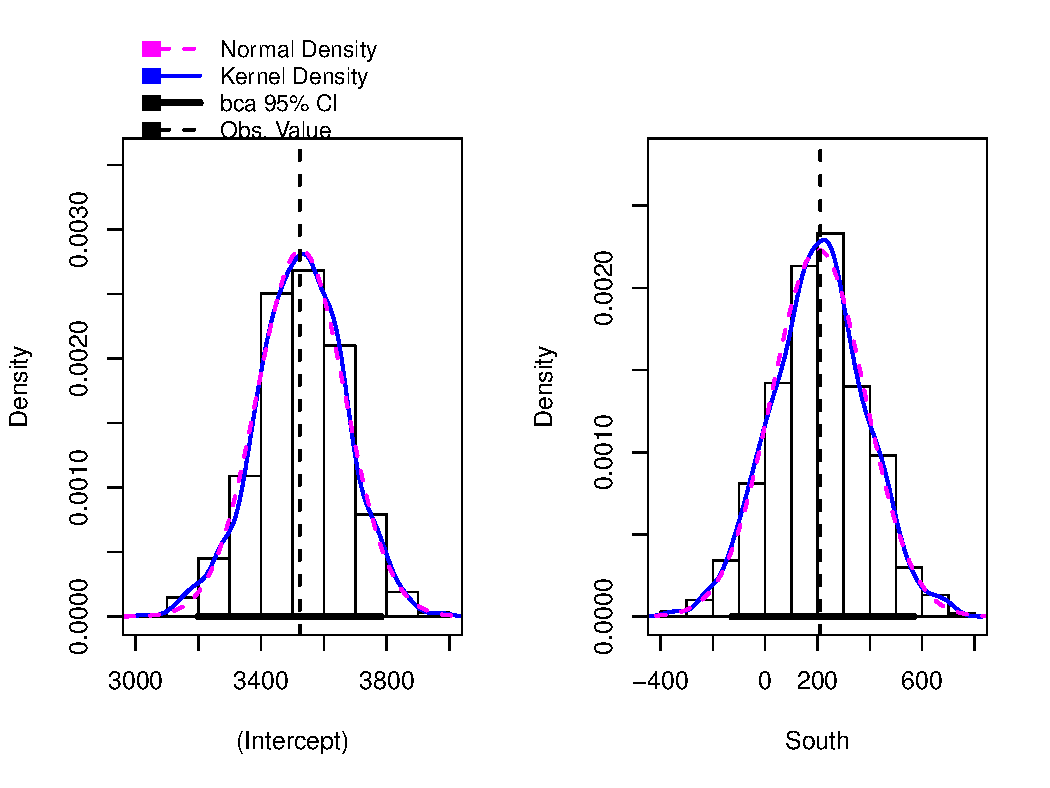
\includegraphics[width=0.55\textwidth]{figure/unnamed-chunk-7-1} 

}



\end{knitrout}
	
\end{frame}




\begin{frame}[fragile,plain]
		\textbf{2.3 Bootstrap CI for mean difference using \texttt{boot} package}
\begin{figure}
	\begin{minipage}[h]{0.40\linewidth}
\begin{knitrout}\tiny
\definecolor{shadecolor}{rgb}{0.969, 0.969, 0.969}\color{fgcolor}\begin{kframe}
\begin{alltt}
\hlkwd{library}\hlstd{(boot)}
\hlcom{# function to obtain deltamu hat}
\hlstd{deltamu} \hlkwb{<-} \hlkwa{function}\hlstd{(}\hlkwc{data}\hlstd{,} \hlkwc{indices}\hlstd{) \{}
        \hlcom{# allows boot to select sample}
        \hlstd{d} \hlkwb{<-} \hlstd{data[indices,]}
        \hlstd{fit} \hlkwb{<-} \hlkwd{lm}\hlstd{(alt} \hlopt{~} \hlstd{South,} \hlkwc{data}\hlstd{=d)}
        \hlkwd{coef}\hlstd{(fit)[}\hlstr{"South"}\hlstd{]}
\hlstd{\}}

\hlstd{results} \hlkwb{<-} \hlstd{boot}\hlopt{::}\hlkwd{boot}\hlstd{(}\hlkwc{data} \hlstd{= depths,}
\hlkwc{statistic} \hlstd{= deltamu,} \hlkwc{R}\hlstd{=}\hlnum{999}\hlstd{)}

\hlstd{results}
\end{alltt}
\begin{verbatim}
## 
## ORDINARY NONPARAMETRIC BOOTSTRAP
## 
## 
## Call:
## boot::boot(data = depths, statistic = deltamu, R = 999)
## 
## 
## Bootstrap Statistics :
##     original    bias    std. error
## t1*   210.75 -0.060188      171.68
\end{verbatim}
\end{kframe}
\end{knitrout}
		
	\end{minipage}
	\hspace{0.4cm}
	\begin{minipage}[h]{0.50\linewidth}
\begin{knitrout}\tiny
\definecolor{shadecolor}{rgb}{0.969, 0.969, 0.969}\color{fgcolor}\begin{kframe}
\begin{alltt}
\hlkwd{plot}\hlstd{(results)}
\end{alltt}
\end{kframe}

{\centering 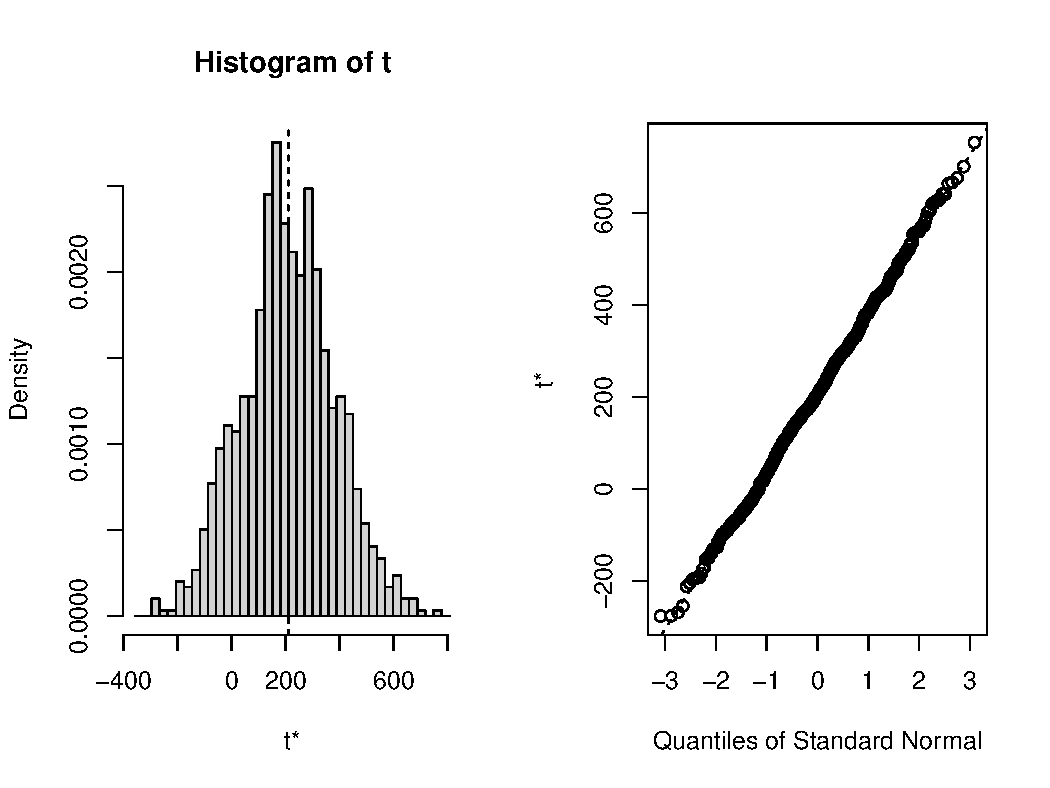
\includegraphics[width=\maxwidth]{figure/unnamed-chunk-9-1} 

}


\begin{kframe}\begin{alltt}
\hlkwd{boot.ci}\hlstd{(results)}
\end{alltt}
\begin{verbatim}
## BOOTSTRAP CONFIDENCE INTERVAL CALCULATIONS
## Based on 999 bootstrap replicates
## 
## CALL : 
## boot.ci(boot.out = results)
## 
## Intervals : 
## Level      Normal              Basic         
## 95%   (-125.7,  547.3 )   (-138.1,  537.1 )  
## 
## Level     Percentile            BCa          
## 95%   (-115.6,  559.6 )   (-106.4,  563.3 )  
## Calculations and Intervals on Original Scale
\end{verbatim}
\end{kframe}
\end{knitrout}
	\end{minipage}
\end{figure}
\end{frame}


\begin{frame}{Permutation Testing}
\begin{itemize}
	\item In testing a null hypothesis we need a test statistic that will have different values under the null hypothesis and the alternatives we	care about 
	\item We then need to compute the sampling distribution of the test	statistic when the null hypothesis is true. For some test statistics	and some null hypotheses this can be done analytically. 
	\item The pvalue is the probability that the test statistic would be at	least as extreme as we observed, if the null hypothesis is true.
	\item A permutation test gives a simple way to compute the sampling	distribution for any test statistic, under the null hypothesis that there is no effect (i.e. South is not a determinant of the mean depth of the ocean)
\end{itemize}
\end{frame}


\begin{frame}{Permutation Testing}
	\begin{itemize}
		\item To estimate the sampling distribution of the test statistic we
		need many samples generated under the strong null hypothesis.
		\item If the null hypothesis is true, changing the exposure would have
		no effect on the outcome. By randomly shuffling the determinants
		we can make up as many data sets as we like.
		\item If the null hypothesis is true, the shuffled data sets should look
		like the real data, otherwise they should look different from the real data.
		\item The ranking of the real test statistic among the shuffled test
		statistics gives a p-value
	\end{itemize}
\end{frame}


\begin{frame}[fragile]{Permutation Testing}
\begin{knitrout}\tiny
\definecolor{shadecolor}{rgb}{0.969, 0.969, 0.969}\color{fgcolor}\begin{kframe}
\begin{alltt}
\hlstd{one.test} \hlkwb{<-} \hlkwa{function}\hlstd{(}\hlkwc{x}\hlstd{,}\hlkwc{y}\hlstd{) \{}
   \hlstd{xstar} \hlkwb{<-} \hlkwd{sample}\hlstd{(x)}
   \hlkwd{mean}\hlstd{(y[xstar}\hlopt{==}\hlnum{1}\hlstd{])} \hlopt{-} \hlkwd{mean}\hlstd{(y[xstar}\hlopt{==}\hlnum{0}\hlstd{])}
\hlstd{\}}

\hlstd{null.dist} \hlkwb{<-} \hlkwd{replicate}\hlstd{(}\hlnum{1000}\hlstd{,} \hlkwd{one.test}\hlstd{(}\hlkwc{x} \hlstd{= depths}\hlopt{$}\hlstd{South,} \hlkwc{y} \hlstd{= depths}\hlopt{$}\hlstd{alt))}
\hlkwd{hist}\hlstd{(null.dist)}
\hlkwd{abline}\hlstd{(}\hlkwc{v}\hlstd{=}\hlkwd{coef}\hlstd{(fit)[}\hlstr{"South"}\hlstd{],} \hlkwc{lwd}\hlstd{=}\hlnum{2}\hlstd{,} \hlkwc{col}\hlstd{=}\hlstr{"blue"}\hlstd{)}
\end{alltt}
\end{kframe}

{\centering 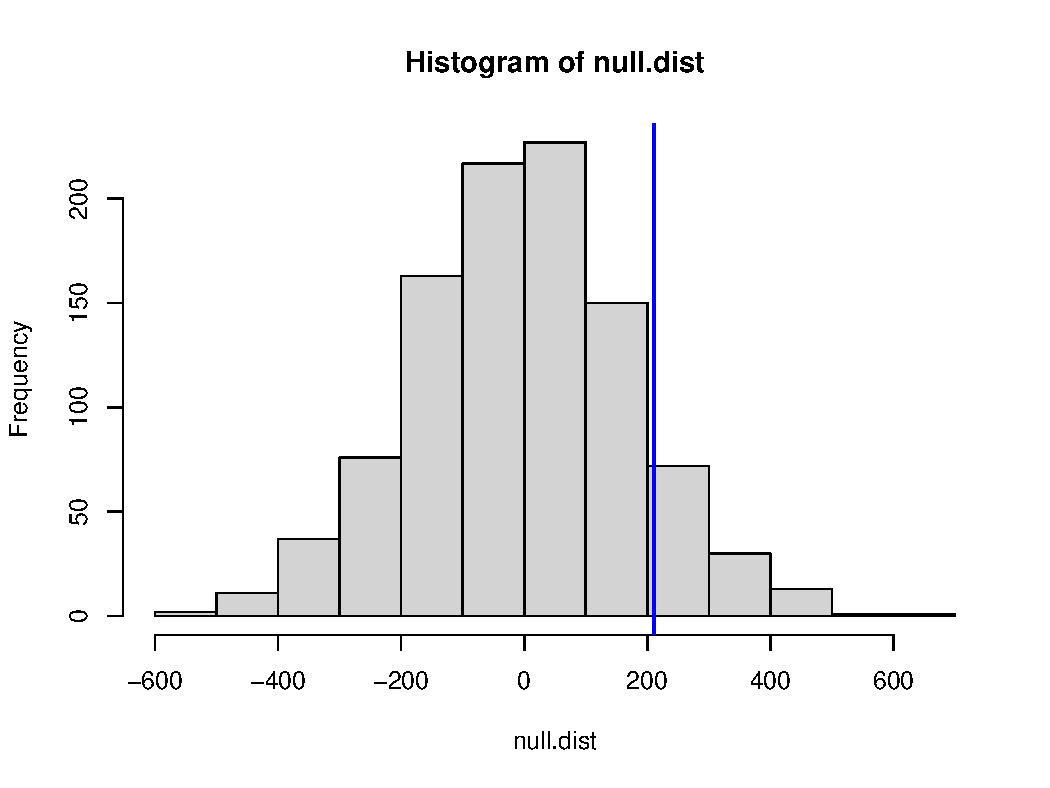
\includegraphics[width=0.5\textwidth]{figure/unnamed-chunk-10-1} 

}


\begin{kframe}\begin{alltt}
\hlkwd{mean}\hlstd{(}\hlkwd{abs}\hlstd{(null.dist)} \hlopt{>} \hlkwd{abs}\hlstd{(}\hlkwd{coef}\hlstd{(fit)[}\hlstr{"South"}\hlstd{]))}
\end{alltt}
\begin{verbatim}
## [1] 0.222
\end{verbatim}
\end{kframe}
\end{knitrout}
\end{frame}




\begin{frame}[fragile,plain]
\vspace*{-1.1in}
\textbf{3. Ratio depth of ocean depths in north vs south hemisphere}
\begin{knitrout}\tiny
\definecolor{shadecolor}{rgb}{0.969, 0.969, 0.969}\color{fgcolor}\begin{kframe}
\begin{alltt}
\hlcom{# note: we are now using glm}
\hlstd{fit} \hlkwb{<-} \hlkwd{glm}\hlstd{(alt} \hlopt{~} \hlstd{South,} \hlkwc{data} \hlstd{= depths,} \hlkwc{family} \hlstd{=} \hlkwd{gaussian}\hlstd{(}\hlkwc{link}\hlstd{=log))}
\hlkwd{print}\hlstd{(}\hlkwd{summary}\hlstd{(fit),} \hlkwc{signif.stars} \hlstd{= F)}
\end{alltt}
\begin{verbatim}
## 
## Coefficients:
##             Estimate Std. Error t value Pr(>|t|)
## (Intercept)   8.1671     0.0347  235.41   <2e-16
## South         0.0581     0.0477    1.22     0.22
## 
## (Dispersion parameter for gaussian family taken to be 2988040)
## 
##     Null deviance: 1193681102  on 399  degrees of freedom
## Residual deviance: 1189239546  on 398  degrees of freedom
## AIC: 7103
## 
## Number of Fisher Scoring iterations: 5
\end{verbatim}
\end{kframe}
\end{knitrout}

\end{frame}


\section{Bootstrap confidence intervals}






\end{document}
